\documentclass{standalone}

\usepackage{pgfplots}
\pgfplotsset{compat=1.11}

\begin{document}
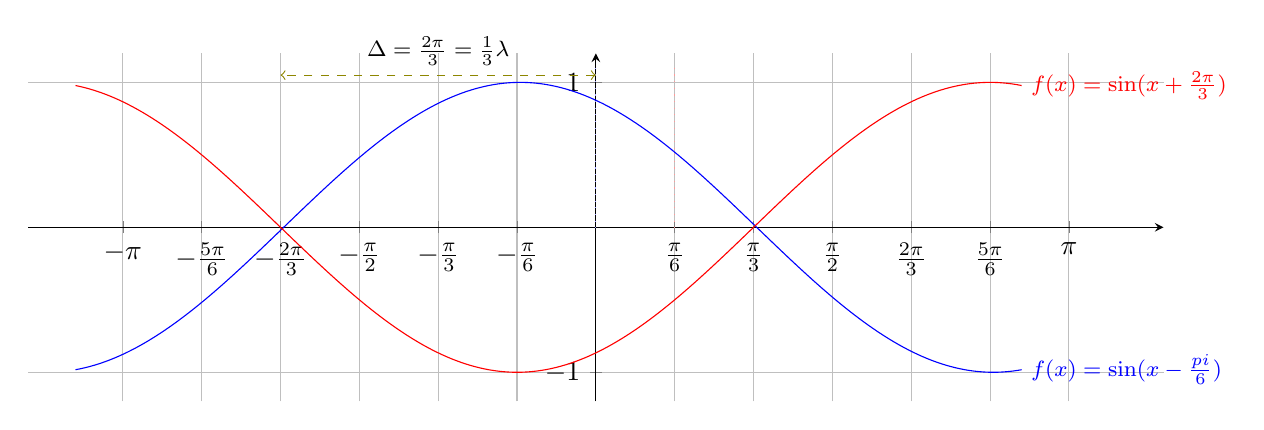
\begin{tikzpicture}
  \begin{axis}[
    grid=both,
    % log ticks with fixed point,
    width=16.0cm,
    height=6cm,
    xmin=-pi,xmax=pi,
    xtick={-pi, -5*pi/6,-4*pi/6,-3*pi/6,-2*pi/6,-pi/6, 0, pi/6, 2*pi/6,3*pi/6,4*pi/6,5*pi/6, pi},
    xticklabels={   
                            $-\pi$,
                            $-\frac{5\pi}{6}$,
                            $-\frac{2\pi}{3}$, 
                            $-\frac{\pi}{2}$, 
                            $-\frac{\pi}{3}$, 
                            $-\frac{\pi}{6}$, 
                            $0$, 
                            $\frac{\pi}{6}$, 
                            $\frac{\pi}{3}$,
                            $\frac{\pi}{2}$,
                            $\frac{2\pi}{3}$,
                            $\frac{5\pi}{6}$,
                            $\pi$,},
    xticklabel style={black},
    trig format plots=rad,
    axis lines = middle,
    enlargelimits,
    clip=false,
    domain=-1.1*pi:0.9*pi,
    samples=200,
    ]
    \addplot[blue] {sin(x+0.33*2*pi)} node[right,pos=1,font=\footnotesize]{$f(x)=\sin(x-\frac{pi}{6})$};
    \addplot[red] {sin(x-1/6*2*pi)} node[right,pos=1,font=\footnotesize]{$f(x)=\sin(x+\frac{2\pi}{3})$};;
    \draw[dotted,blue!40] (axis cs: 0,1.1) -- (axis cs: 0,0);
    \draw[dotted,red!40] (axis cs: pi/6,1.1) -- (axis cs: pi/6,0);
    \draw[dashed,olive,<->] (axis cs: 0,1.05) -- node[above,text=black,font=\footnotesize]{$\Delta = \frac{2\pi}{3}=\frac{1}{3}\lambda$}(axis cs: -4*pi/6,1.05);
  \end{axis}
\end{tikzpicture}
\end{document}